%%%%%%%%%%%%%%%%%%%%%%%%%%%%%%%%%%%%%%%%%%%%%%%%%%%
%
%  New template code for TAMU Theses and Dissertations starting Fall 2012.  
%  For more info about this template or the 
%  TAMU LaTeX User's Group, see http://www.howdy.me/.
%
%  Author: Wendy Lynn Turner 
%	 Version 1.0 
%  Last updated 8/5/2012
%
%%%%%%%%%%%%%%%%%%%%%%%%%%%%%%%%%%%%%%%%%%%%%%%%%%%
%%%                           SECTION V
%%%%%%%%%%%%%%%%%%%%%%%%%%%%%%%%%%%%%%%%%%%%%%%%%%%
\chapter{\uppercase {FEM Basis Functions for Unstructured Polytopes}}
\label{sec::BF}

%%%%%%%%%%%%%%%%%%%%%%%%%%%%%%%%%%%%%%%%%%%%%%%%%%%
%%%   Section - 2D
\section{Two-Dimensional Basis Functions on Polygons}
\label{sec::BF_2D}



\begin{figure}[hbt]
\centering
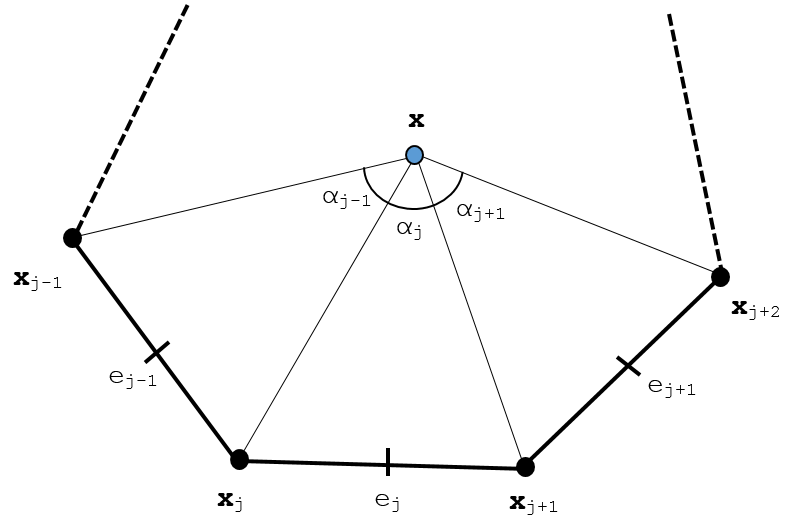
\includegraphics[width=0.65\textwidth]{figures/sec_BF/ref_polygon.png}
\caption{Arbitrary polygon with geometric properties used for 2D basis function generation.}
\label{fig::BF_2D_ref_polygon}
\end{figure}

%%%%%%%%%%%%%%%%%%%%%%%%%%%%%%%%%%%%%%%%%%%%%%%%%%%
%%%   SubSection - Linear Basis Functions
\subsection{Linearly-Complete 2D Basis Functions}
\label{sec::BF_2D_Linear}

In this dissertation, all 1st-order, two-dimensional basis functions for a cell will obey the properties for barycentric coordinates. They will form a {\em partition of unity},

\begin{equation}
\sum_{i=1}^{N_K} b_i (\vec{x})  =  1;
\label{eq::BF_linear_interp_partition}
\end{equation}

\noindent coordinate interpolation will result from an {\em affine combination} of the vertices,

\begin{equation}
\sum_{i=1}^{N_K} b_i(\vec{x}) \vec{x}_i  =  \vec{x};
\label{eq::BF_linear_interp_affine}
\end{equation}

\noindent and they will satisfy the {\em Lagrange property},

\begin{equation}
b_i (\vec{x}_j) = \delta_{ij}.
\label{eq::BF_linear_interp_lagrange}
\end{equation}

\noindent $N_K$ is again the number of spatial degrees with measure in element $K$. Using the {\em partition of unity} of Eq. (\ref{eq::BF_linear_interp_partition}), we can rewrite Eqs. (\ref{eq::BF_linear_interp_partition}-\ref{eq::BF_linear_interp_affine}) into a separate, compact, vectorized form for completeness

\begin{equation}
\sum_{i=1}^{N_K}  b_i (\vec{x}) \vec{c}_{i,1}(\vec{x}) = \vec{q}_1 ,
\label{eq::BF_linear_interp_req_vector}
\end{equation}

\noindent where $\vec{c}_{i,1}(\vec{x})$ and $\vec{q}_1$ are the lineary-complete constraint and equivalence terms, respectively. These terms are simply:

\begin{equation}
\vec{c}_{i,1}(\vec{x}) = \left[
\begin{array}{c}
1 \\
x_i - x \\
y_i - y
\end{array} \right]
  \qquad \text{and} \qquad \vec{q}_1 = \left[
\begin{array}{c}
1 \\
0 \\
0
\end{array} \right],
\label{eq::BF_linear_constraint_terms}
\end{equation}

\noindent respectively.

%%%%%%%%%%%%%%%%%%%%%%%%%%%%%%%%%%%%%%%%%%%%%%%%%%%
%%%   SubSubSection - Linear
\subsubsection{Linear and BiLinear Basis Functions}
\label{sec::BF_2D_Linear_LDandBLD}

Before presenting basis function sets applicable to polytope finite elements, we first provide two basis functions that are exact 

\begin{equation}
\label{eq::2D_lin_basis_functions}
\begin{aligned}
	b_1(r,s) & = 1-r-s \\
	b_2(r,s) & = r \\
	b_3(r,s) & = s 
\end{aligned}
\end{equation}

\noindent 

and

\begin{equation}
\label{eq::BiL_basis_functions}
\begin{aligned}
	b_1(r,s) & = (1-r)(1-s) \\
	b_2(r,s) & = r(1-s) \\
	b_3(r,s) & = rs \\
	b_4(r,s) & = (1-r)s
\end{aligned}
\end{equation}


%%%%%%%%%%%%%%%%%%%%%%%%%%%%%%%%%%%%%%%%%%%%%%%%%%%
%%%   SubSection - Wachspress
\subsubsection{Wachspress Rational Basis Functions}
\label{sec::BF_2D_Linear_Wachspress}

%%%%%%%%%%%%%%%%%%%%%%%%%%%%%%%%%%%%%%%%%%%%%%%%%%%
%%%   SubSection - Mean Value
\subsubsection{Mean Value Basis Functions}
\label{sec::BF_2D_Linear_MV}

%%%%%%%%%%%%%%%%%%%%%%%%%%%%%%%%%%%%%%%%%%%%%%%%%%%
%%%   SubSection - Metric
\subsubsection{Metric Basis Functions}
\label{sec::BF_2D_Linear_Metric}

%%%%%%%%%%%%%%%%%%%%%%%%%%%%%%%%%%%%%%%%%%%%%%%%%%%
%%%   SubSection - Maximum Entropy
\subsubsection{Maximum Entropy Basis Functions}
\label{sec::BF_2D_Linear_ME}

%%%%%%%%%%%%%%%%%%%%%%%%%%%%%%%%%%%%%%%%%%%%%%%%%%%
%%%   SubSection - PWL
\subsubsection{Piecewise Linear (PWL) Basis Functions}
\label{sec::BF_2D_Linear_PWL}

\begin{equation}
\label{eq::PWL_2D}
	b_j (x,y) = t_j (x,y) + \alpha_j^K t_c (x,y)
\end{equation}

\noindent $t_j$ is the standard 2D linear function with unity at vertex $j$ that linearly decreases to zero to the cell center and each adjoining vertex. $t_c$ is the 2D cell ``tent'' function which is unity at the cell center and linearly decreases to zero to each cell vertex. $\alpha_{j}^{K}$ is the weight parameter for vertex $j$ in cell $K$. 



%%%%%%%%%%%%%%%
% Begin::2D PWL basis function plots
\pagebreak
\begin{figure}
\label{fig::2D_PWL_unit_square_basis_functions}
\centering
	\begin{subfigure}[b]{0.48\textwidth}
		\centering
		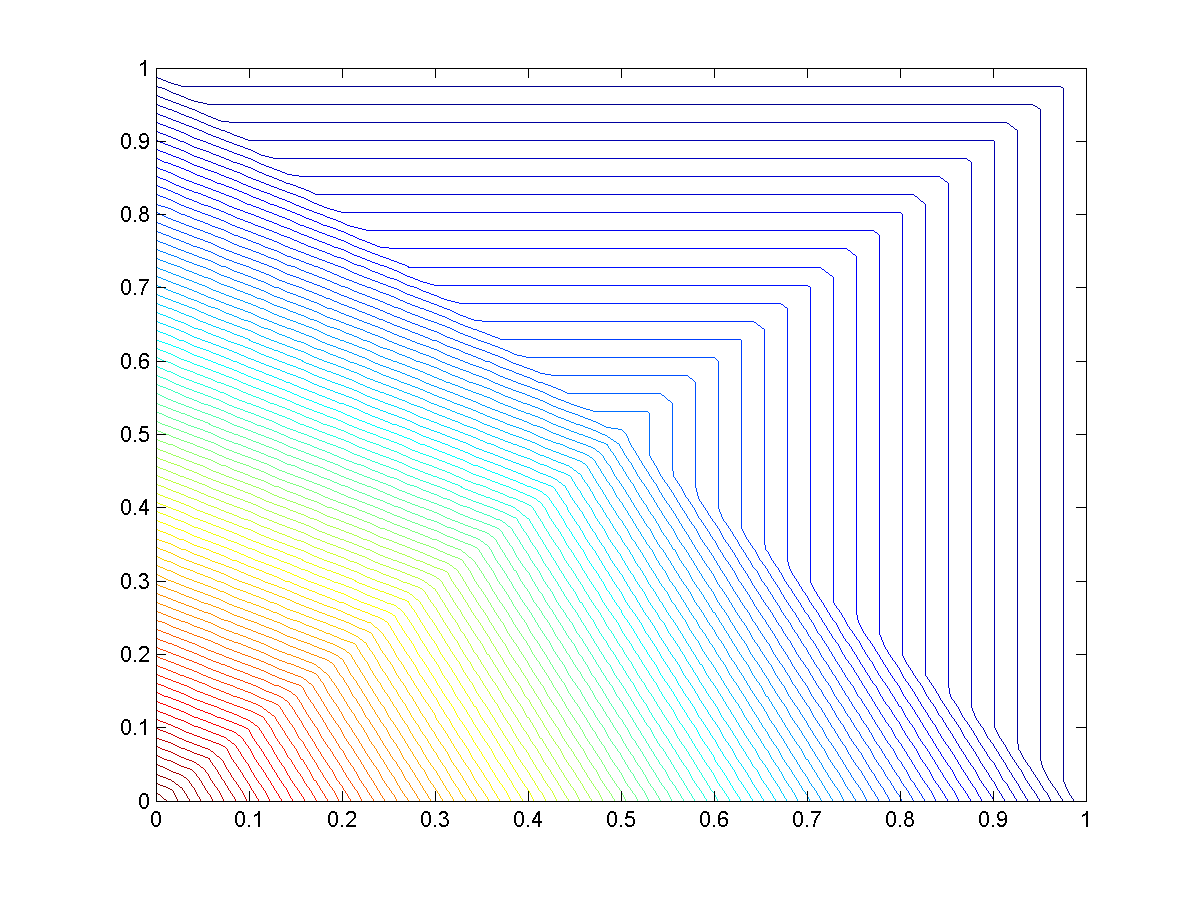
\includegraphics[width=\textwidth]{figures/sec_BF/PWL_square_contour_1.png}
		\caption{}
	\end{subfigure}
	\hfill
	\begin{subfigure}[b]{0.48\textwidth}
		\centering
		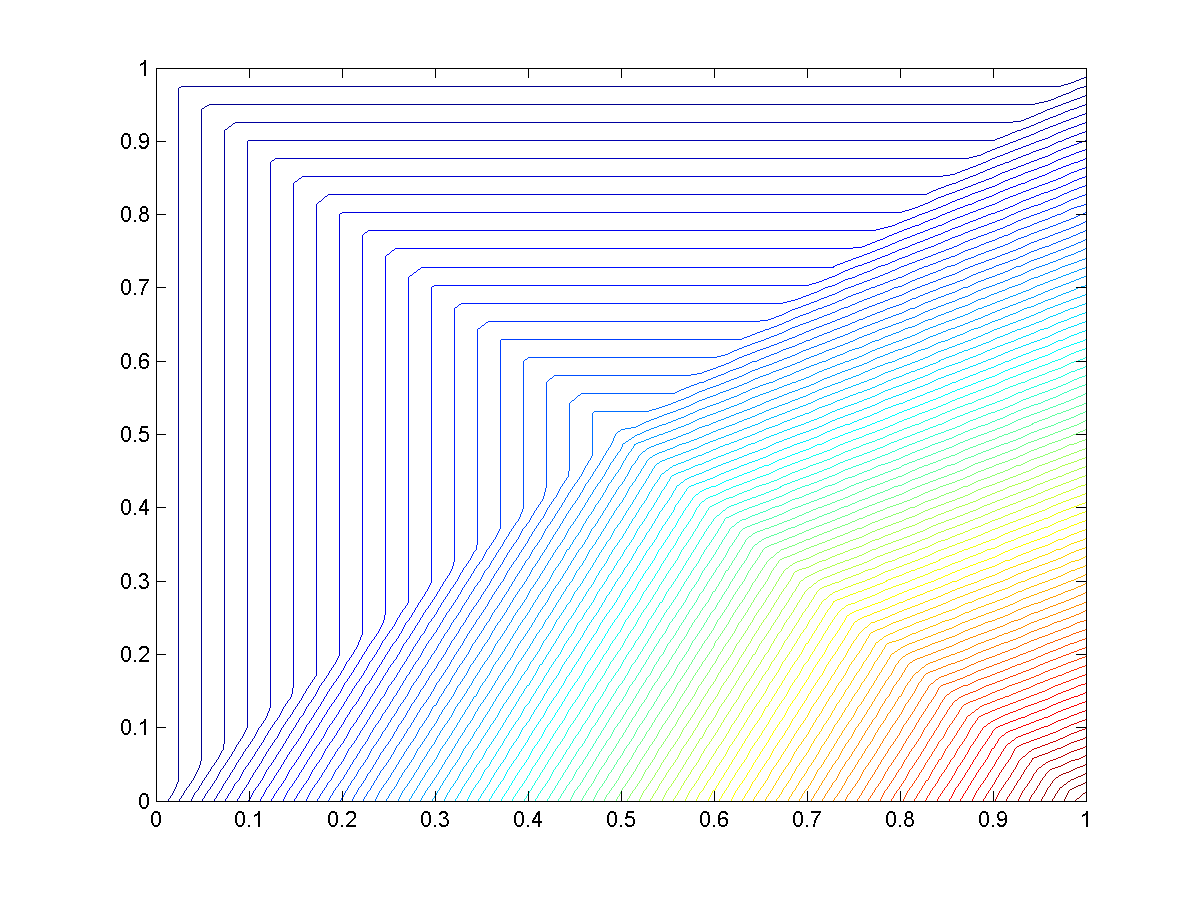
\includegraphics[width=\textwidth]{figures/sec_BF/PWL_square_contour_2.png}
		\caption{}
	\end{subfigure}
	\vfill
	\begin{subfigure}[b]{0.48\textwidth}
		\centering
		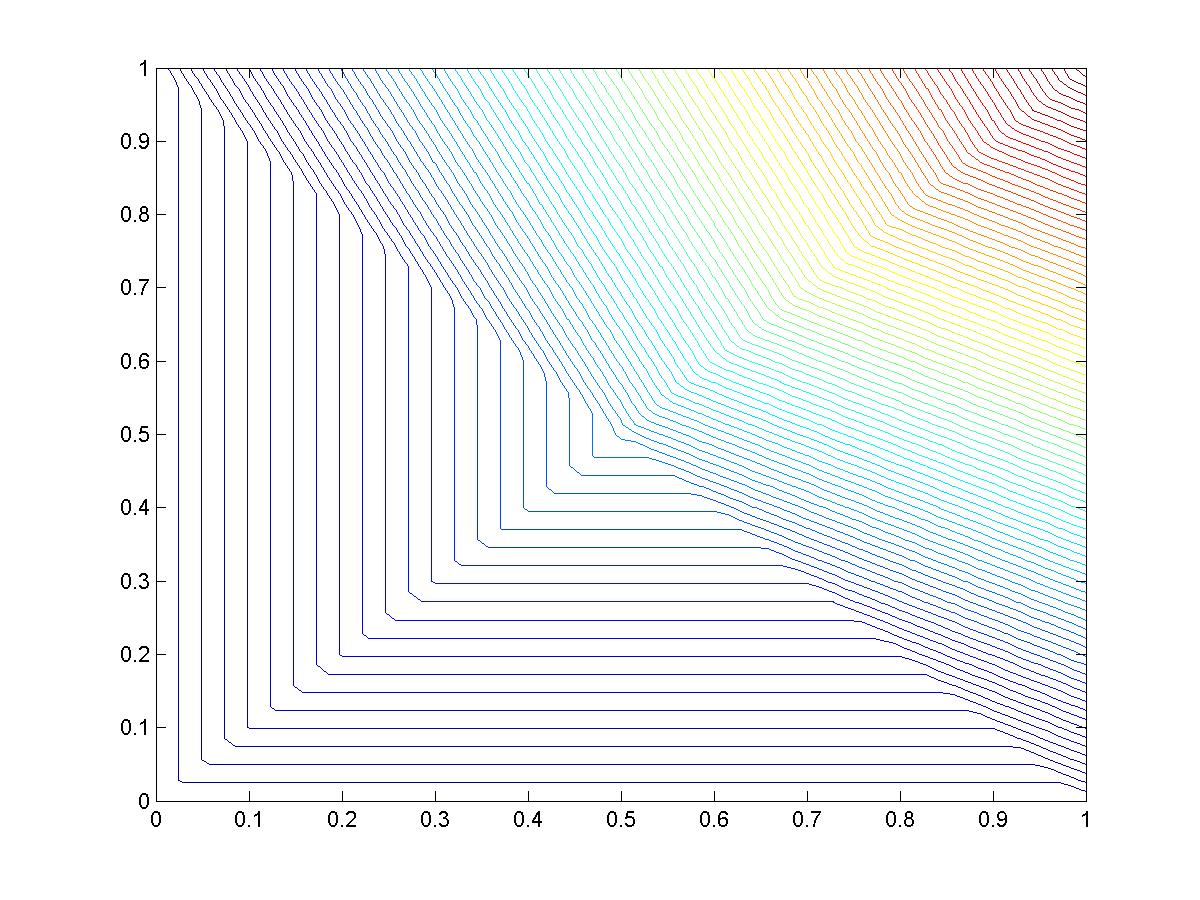
\includegraphics[width=\textwidth]{figures/sec_BF/PWL_square_contour_3.png}
		\caption{}
	\end{subfigure}
	\hfill
	\begin{subfigure}[b]{0.48\textwidth}
		\centering
		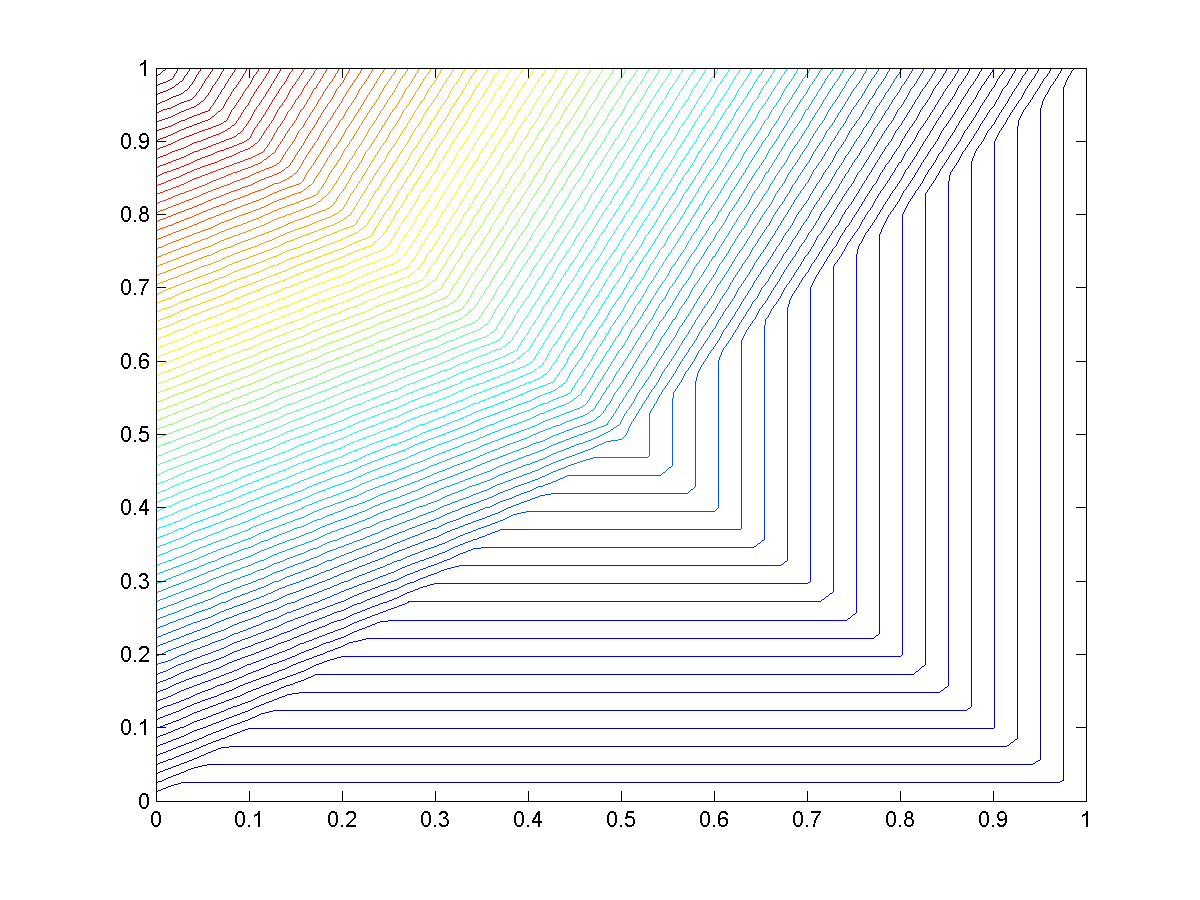
\includegraphics[width=\textwidth]{figures/sec_BF/PWL_square_contour_4.png}
		\caption{}
	\end{subfigure}
\caption{Contour plots of the PWL basis functions on the unit square for the vertices located at: (a) (0,0), (b) (1,0), (c) (1,1), and (d) (0,1).}
\end{figure}

\begin{figure}
\label{fig::2D_pentagon_vertices}
\centering
	\begin{subfigure}[b]{0.40\textwidth}
		\centering
		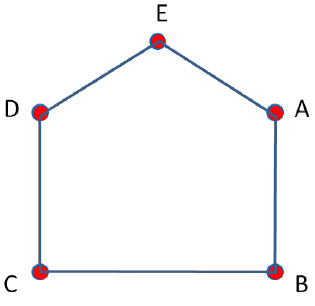
\includegraphics[width=\textwidth]{figures/sec_BF/reg_pent_verts.png}
		\caption{}
	\end{subfigure}
	\hfill
	\begin{subfigure}[b]{0.40\textwidth}
		\centering
		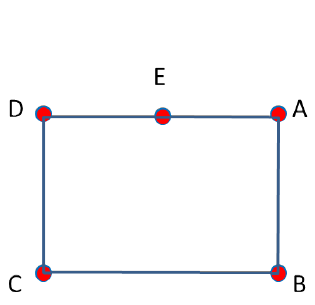
\includegraphics[width=\textwidth]{figures/sec_BF/deg_pent_verts.png}
		\caption{}
	\end{subfigure}
\caption{Vertex structure for a (a) regular pentagonal cell and a (b) degenerate pentagonal cell.}
\end{figure}

\begin{figure}
\label{fig::2D_PWL_pentagon_basis_functions_contour}
\centering
	\begin{subfigure}[b]{0.48\textwidth}
		\centering
		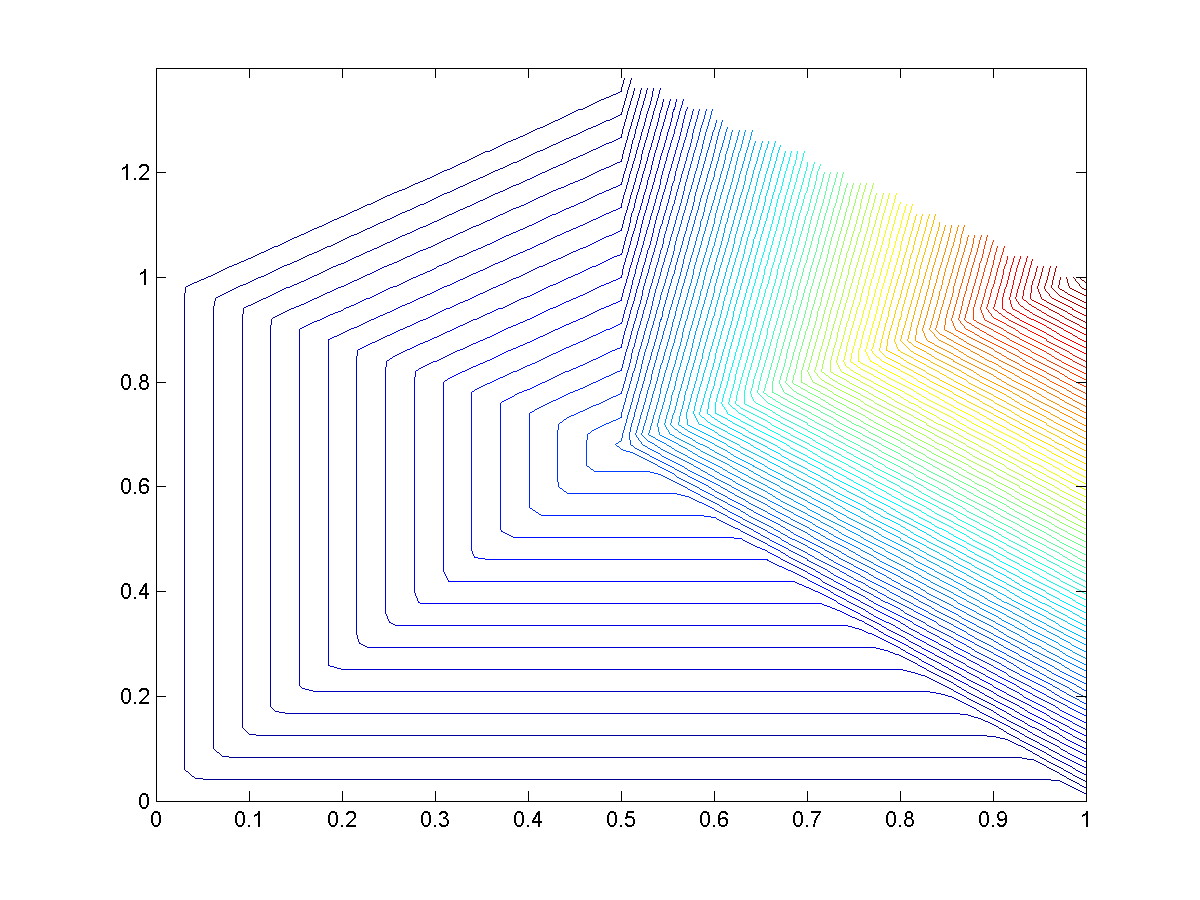
\includegraphics[width=\textwidth]{figures/sec_BF/PWL_rpent_contour_A.png}
		\caption{}
	\end{subfigure}
	\hfill
	\begin{subfigure}[b]{0.48\textwidth}
		\centering
		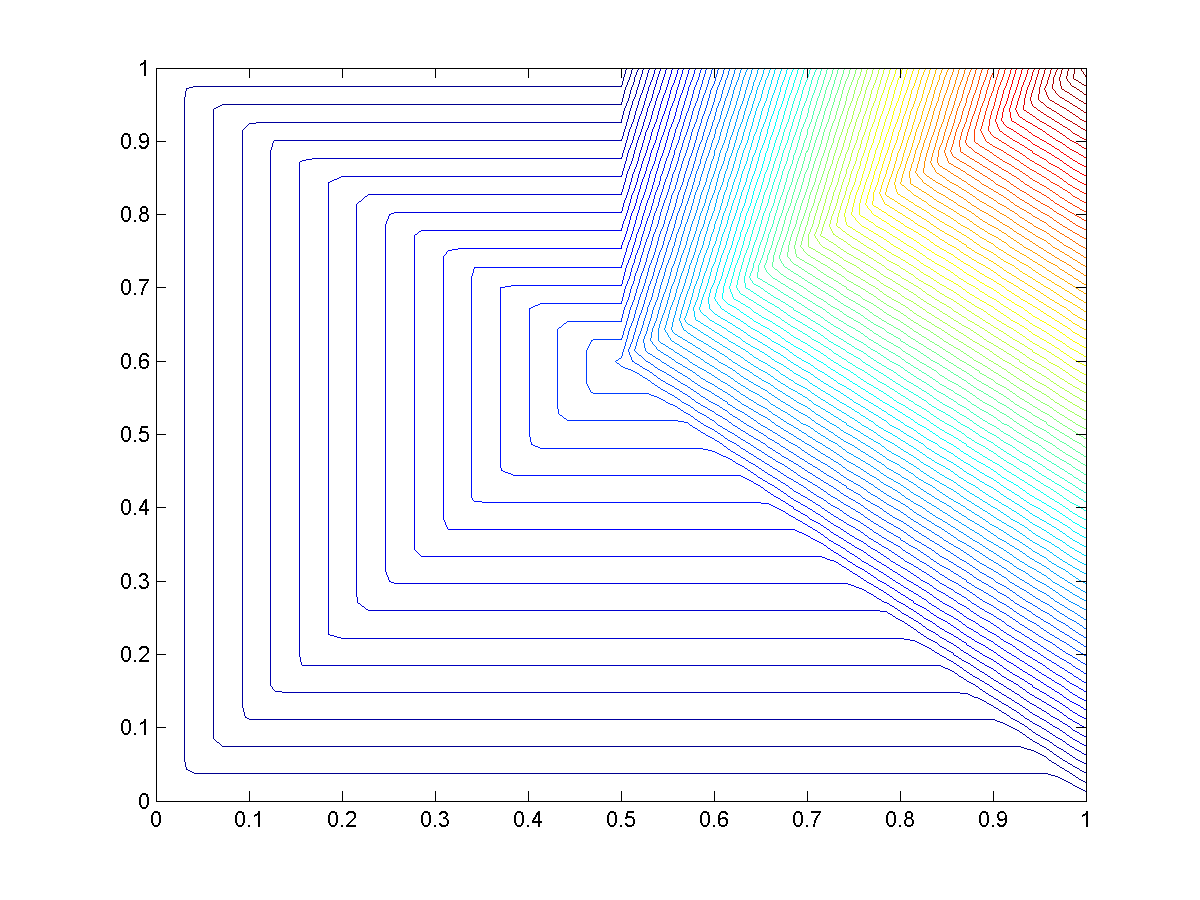
\includegraphics[width=\textwidth]{figures/sec_BF/PWL_dpent_contour_A.png}
		\caption{}
	\end{subfigure}
	\vfill
	\begin{subfigure}[b]{0.48\textwidth}
		\centering
		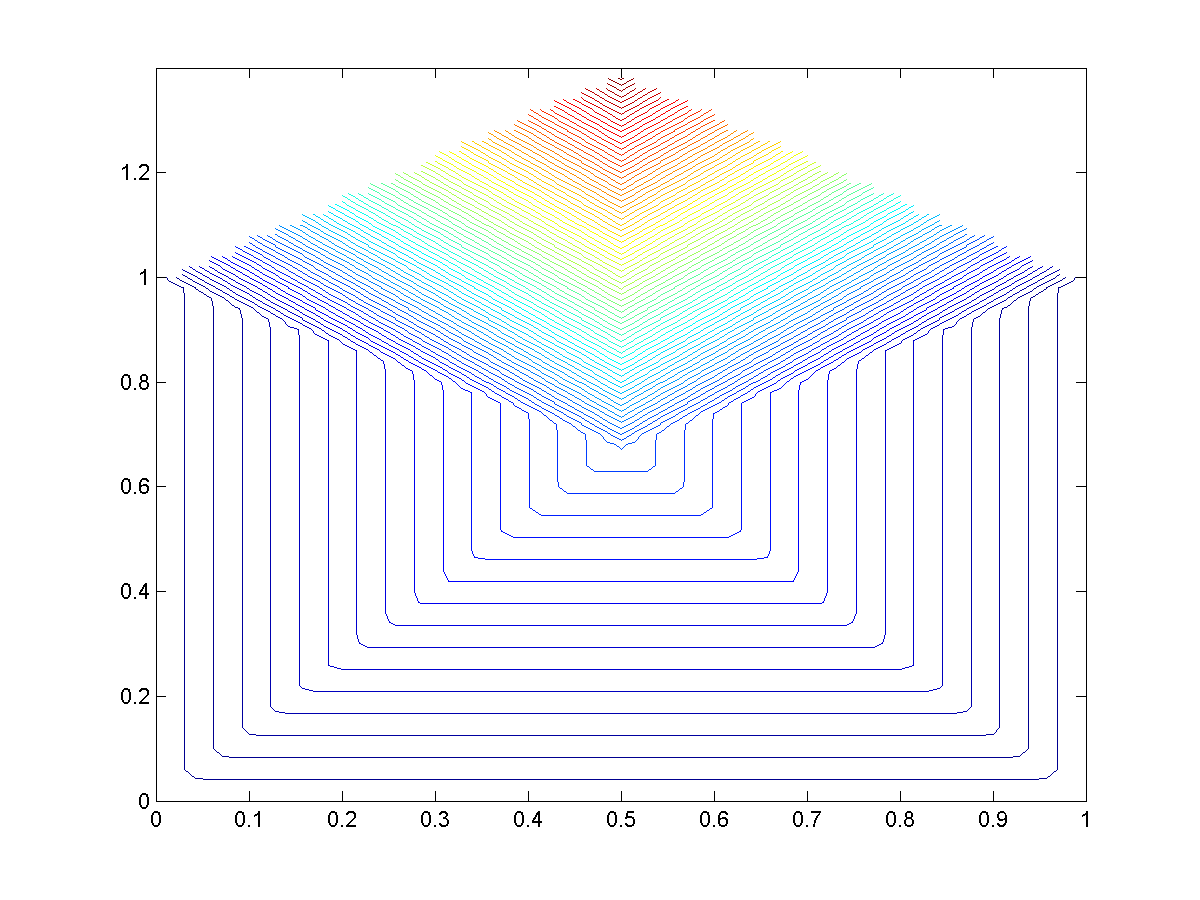
\includegraphics[width=\textwidth]{figures/sec_BF/PWL_rpent_contour_E.png}
		\caption{}
	\end{subfigure}
	\hfill
	\begin{subfigure}[b]{0.48\textwidth}
		\centering
		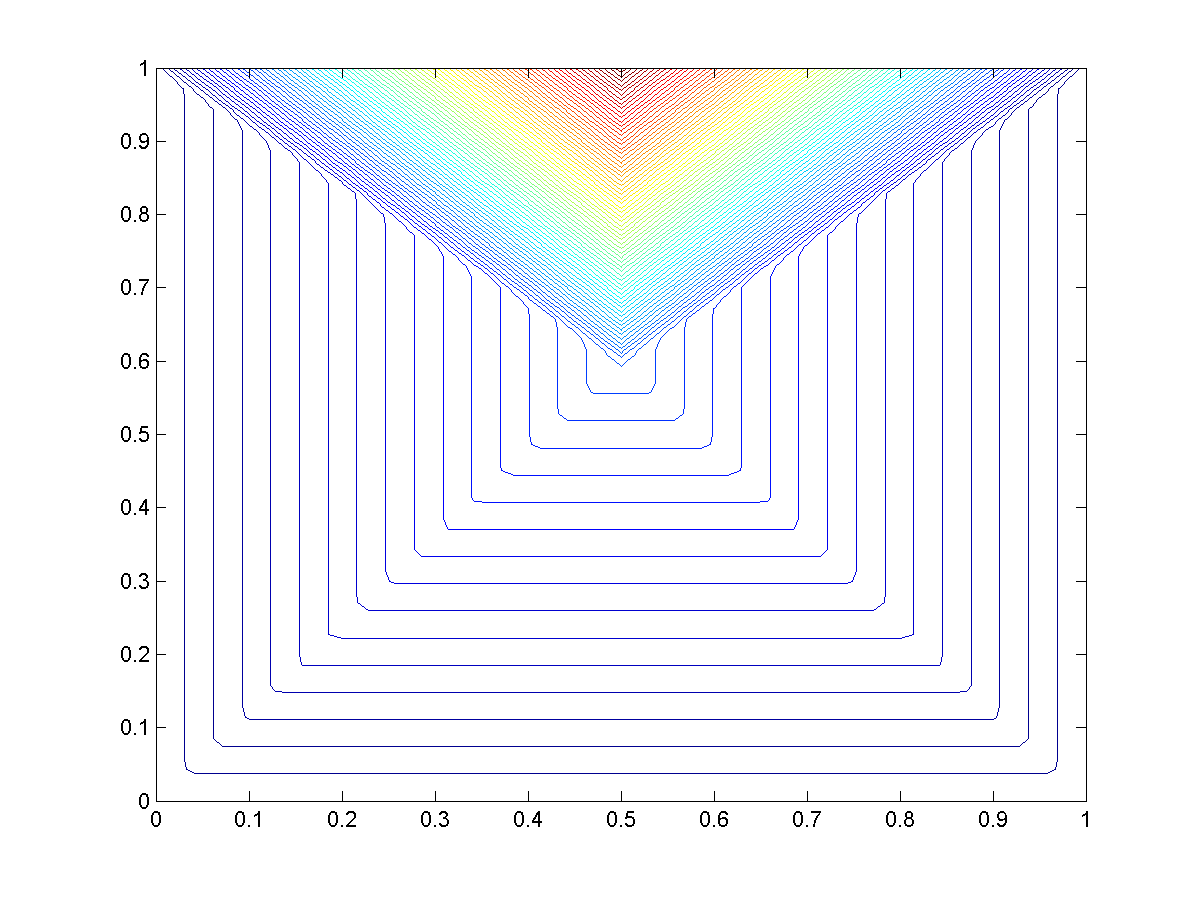
\includegraphics[width=\textwidth]{figures/sec_BF/PWL_dpent_contour_E.png}
		\caption{}
	\end{subfigure}
\caption{Contour plots of the PWL basis functions for a regular pentagon: (a) and (c) as well as a degenerate pentagon: (b) and (d).}
\end{figure}

\begin{figure}
\label{fig::2D_PWL_pentagon_basis_functions_plot}
\centering
	\begin{subfigure}[b]{0.48\textwidth}
		\centering
		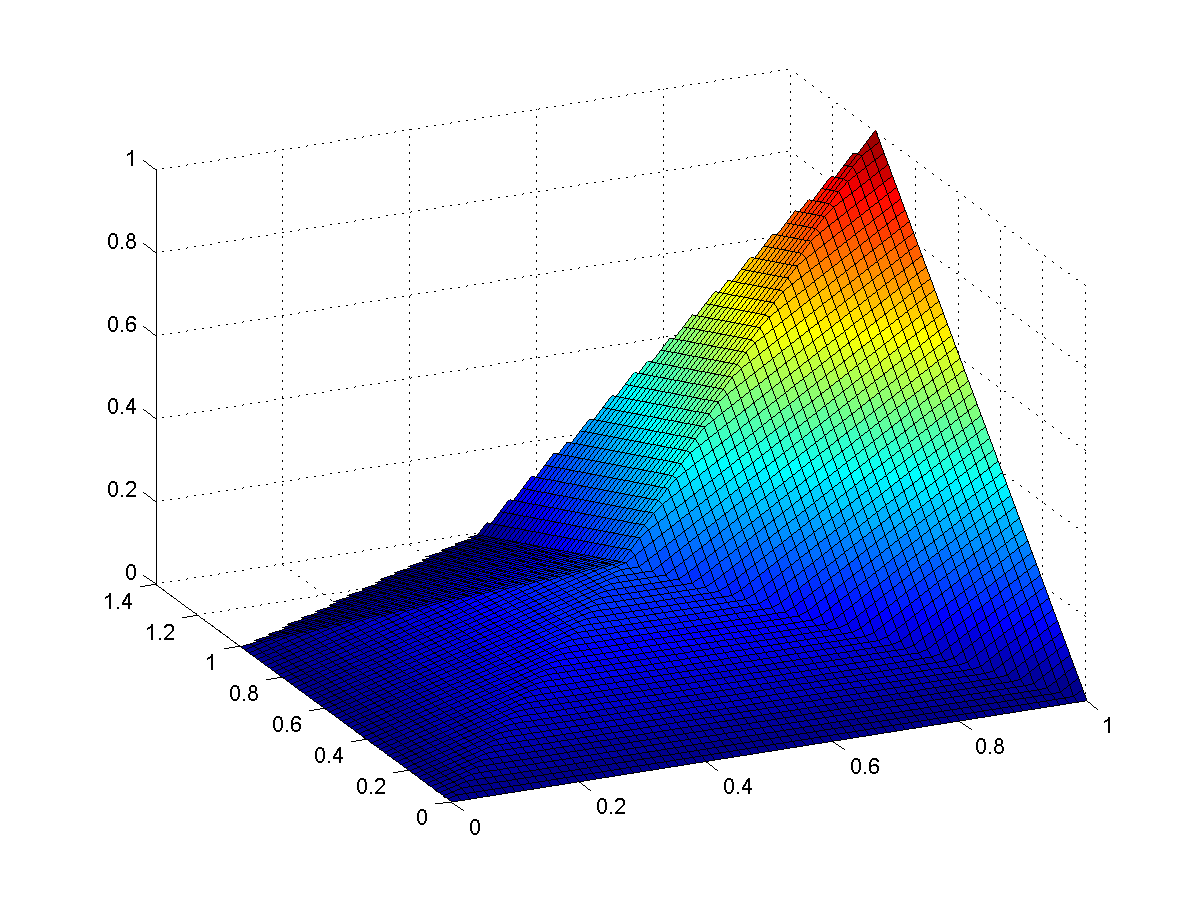
\includegraphics[width=\textwidth]{figures/sec_BF/PWL_rpent_plot_A.png}
		\caption{}
	\end{subfigure}
	\hfill
	\begin{subfigure}[b]{0.48\textwidth}
		\centering
		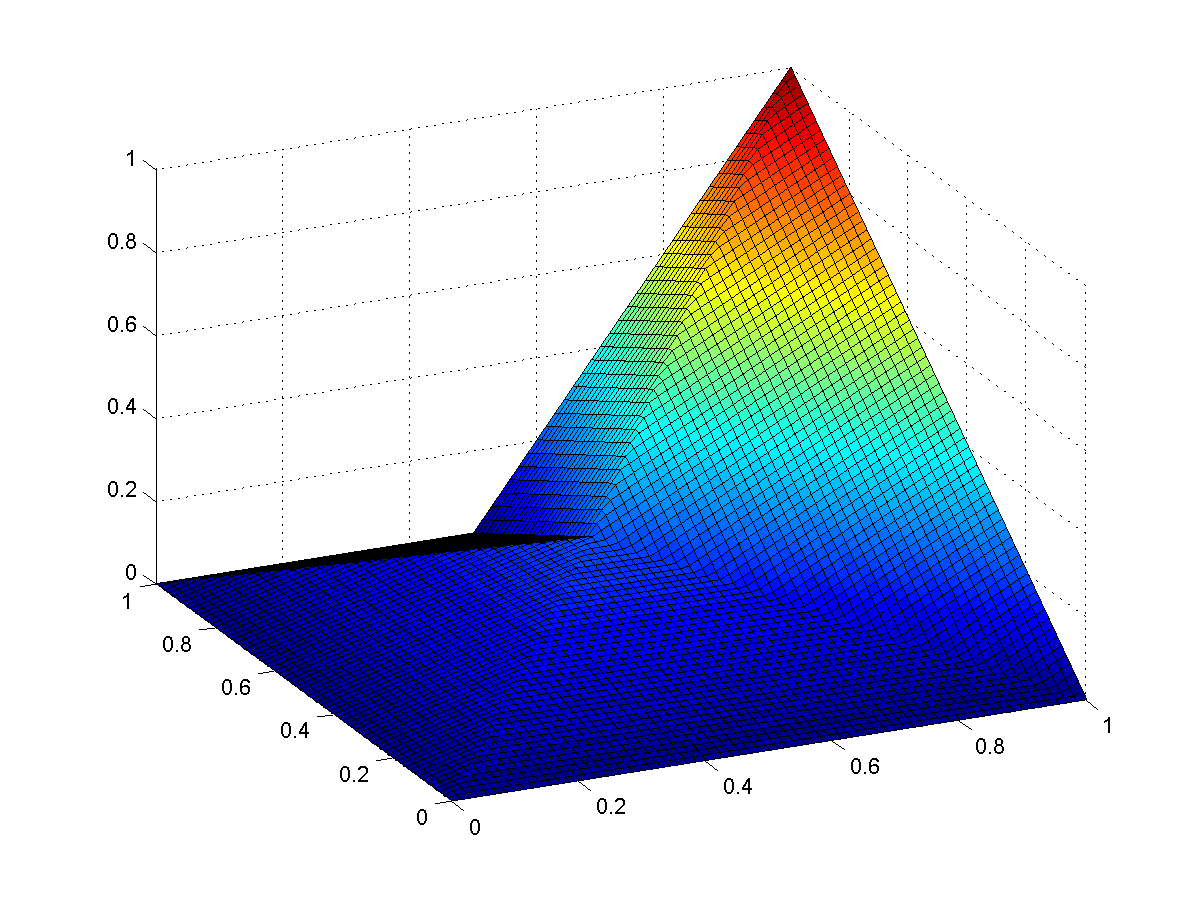
\includegraphics[width=\textwidth]{figures/sec_BF/PWL_dpent_plot_A.png}
		\caption{}
	\end{subfigure}
	\vfill
	\begin{subfigure}[b]{0.48\textwidth}
		\centering
		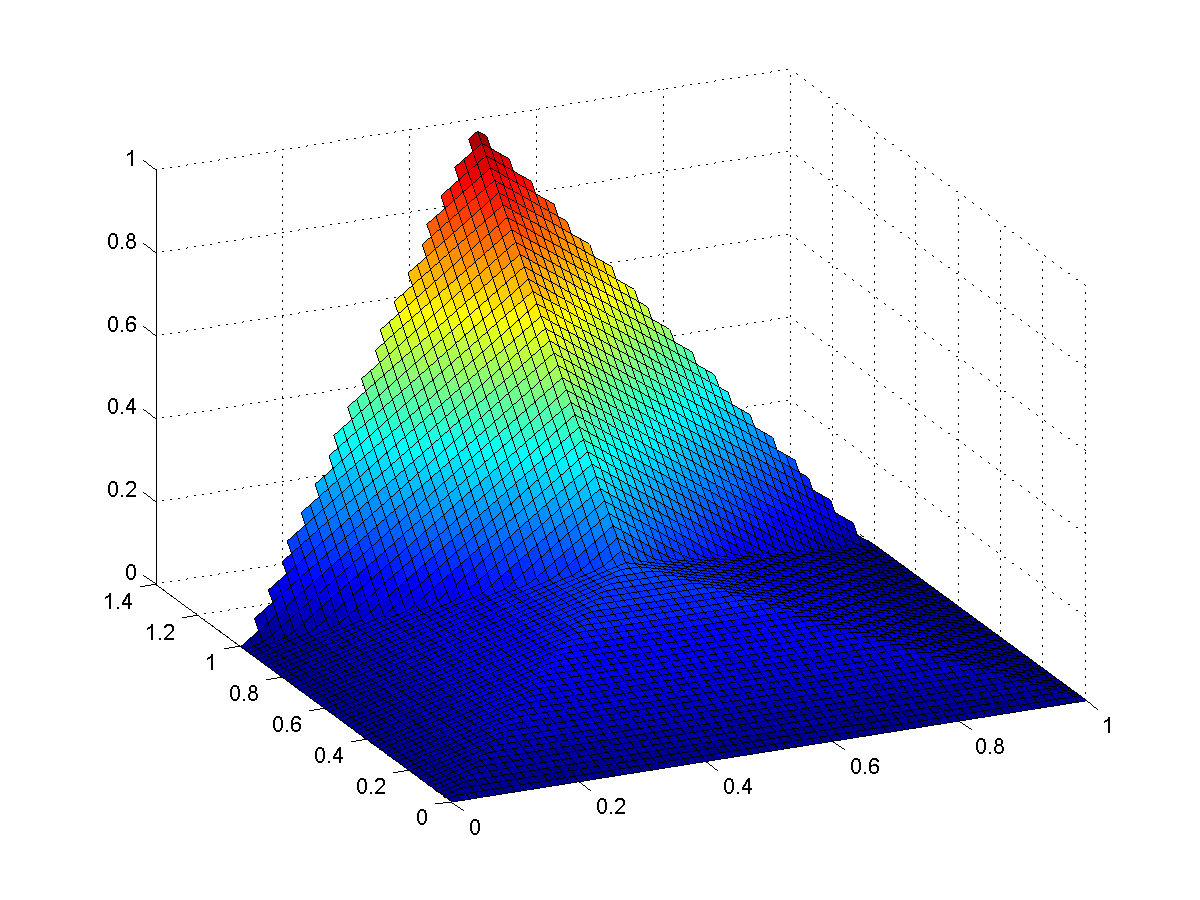
\includegraphics[width=\textwidth]{figures/sec_BF/PWL_rpent_plot_E.png}
		\caption{}
	\end{subfigure}
	\hfill
	\begin{subfigure}[b]{0.48\textwidth}
		\centering
		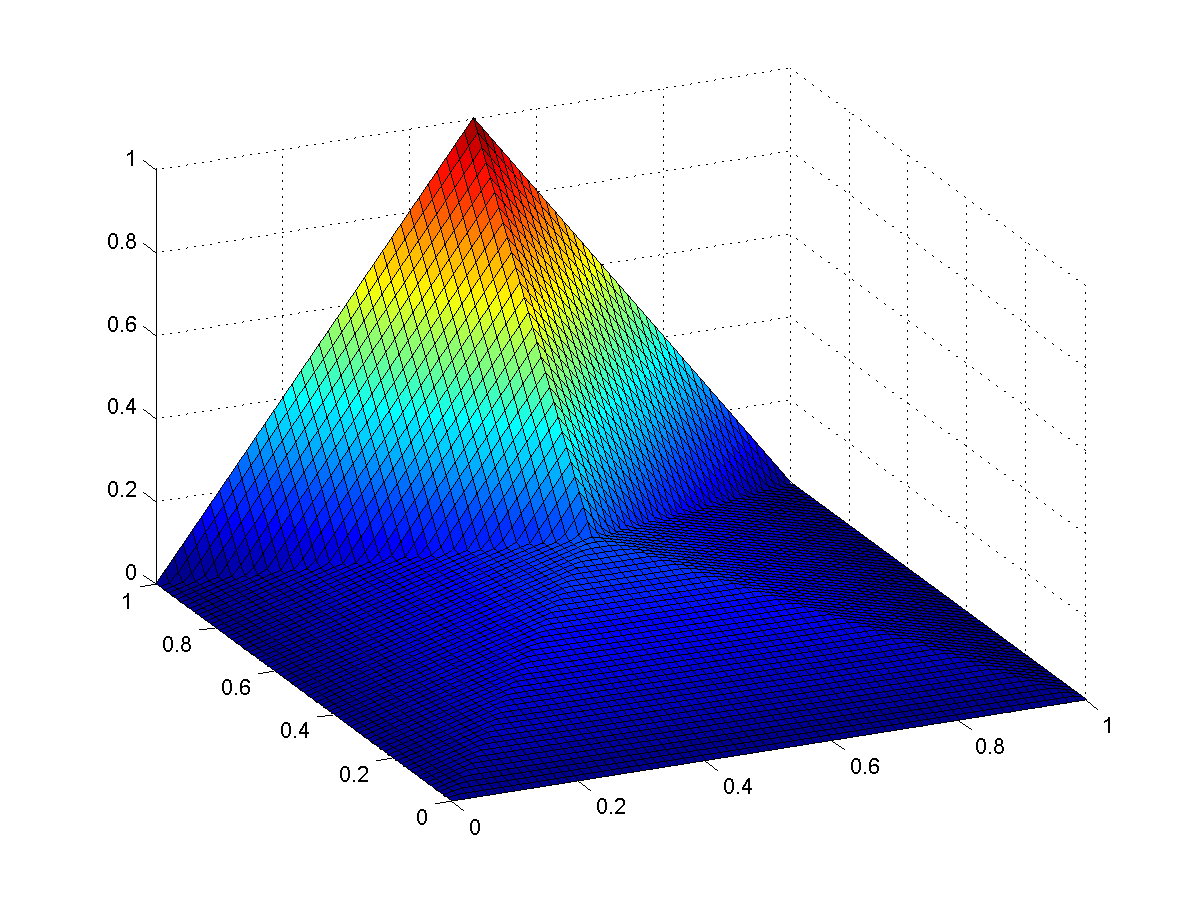
\includegraphics[width=\textwidth]{figures/sec_BF/PWL_dpent_plot_E.png}
		\caption{}
	\end{subfigure}
\caption{Plots of the PWL basis functions for a regular pentagon: (a) and (c) as well as a degenerate pentagon: (b) and (d).}
\end{figure}
% End::2D PWL basis function plots
%%%%%%%%%%%%%%%

%%%%%%%%%%%%%%%%%%%%%%%%%%%%%%%%%%%%%%%%%%%%%%%%%%%
%%%   SubSubSection - 2D linear summary
\subsubsection{Summary of Linear Basis Functions on Polygons}
\label{sec::BF_2D_Linear_Summary}

%%%%%%%%%%%%%%%%%%%%%%%%%%%%%%%%%%%%%%%%%%%%%%%%%%%
%%%   Section - Quadratic Basis Functions
\subsection{Quadratically-Complete 2D Basis Functions}
\label{sec::BF_2D_Quadratic}

\begin{gather}
	 \sum_{i=1}^{N_K} b_i (\vec{x})  =  1 \\
	\sum_{i=1}^{N_K} b_i(\vec{x}) \vec{x}_i  =  \vec{x} \\
	\sum_{i=1}^{N_K} \sum_{j=1}^{N_K} \mu _{i,j}  \left(   \frac{\vec{x}_i \otimes \vec{x}_j +\vec{x}_j \otimes \vec{x}_i }{2}  \right)  = \vec{x} \otimes \vec{x}
\label{eq::quadratic_interp_requirements}
\end{gather}

\noindent where $\mu_{i,j}$ is a weight function corresponding to particular basis function pairings.

%%%%%%%%%%%%%%%%%%%%%%%%%%%%%%%%%%%%%%%%%%%%%%%%%%%
%%%   SubSection - BiL/TriL
\subsubsection{Serendipity Bilinear and Trilinear Basis Functions}
\label{sec::BF_Quadratic_BiLTriL}

%%%%%%%%%%%%%%%%%%%%%%%%%%%%%%%%%%%%%%%%%%%%%%%%%%%
%%%   Section - 3D
\section{Three-Dimensional Basis Functions on Polyhedra}
\label{sec::BF_3D}



%%%%%%%%%%%%%%%%%%%%%%%%%%%%%%%%%%%%%%%%%%%%%%%%%%%
%%%   SubSection - 3D Lin/TriL
\subsection{3D Linear and TriLinear Basis Functions}
\label{sec::BF_3D_TriL}

\begin{figure}
\centering
	\begin{subfigure}[b]{0.45\textwidth}
		\centering
		\label{subfig::unit_square}
		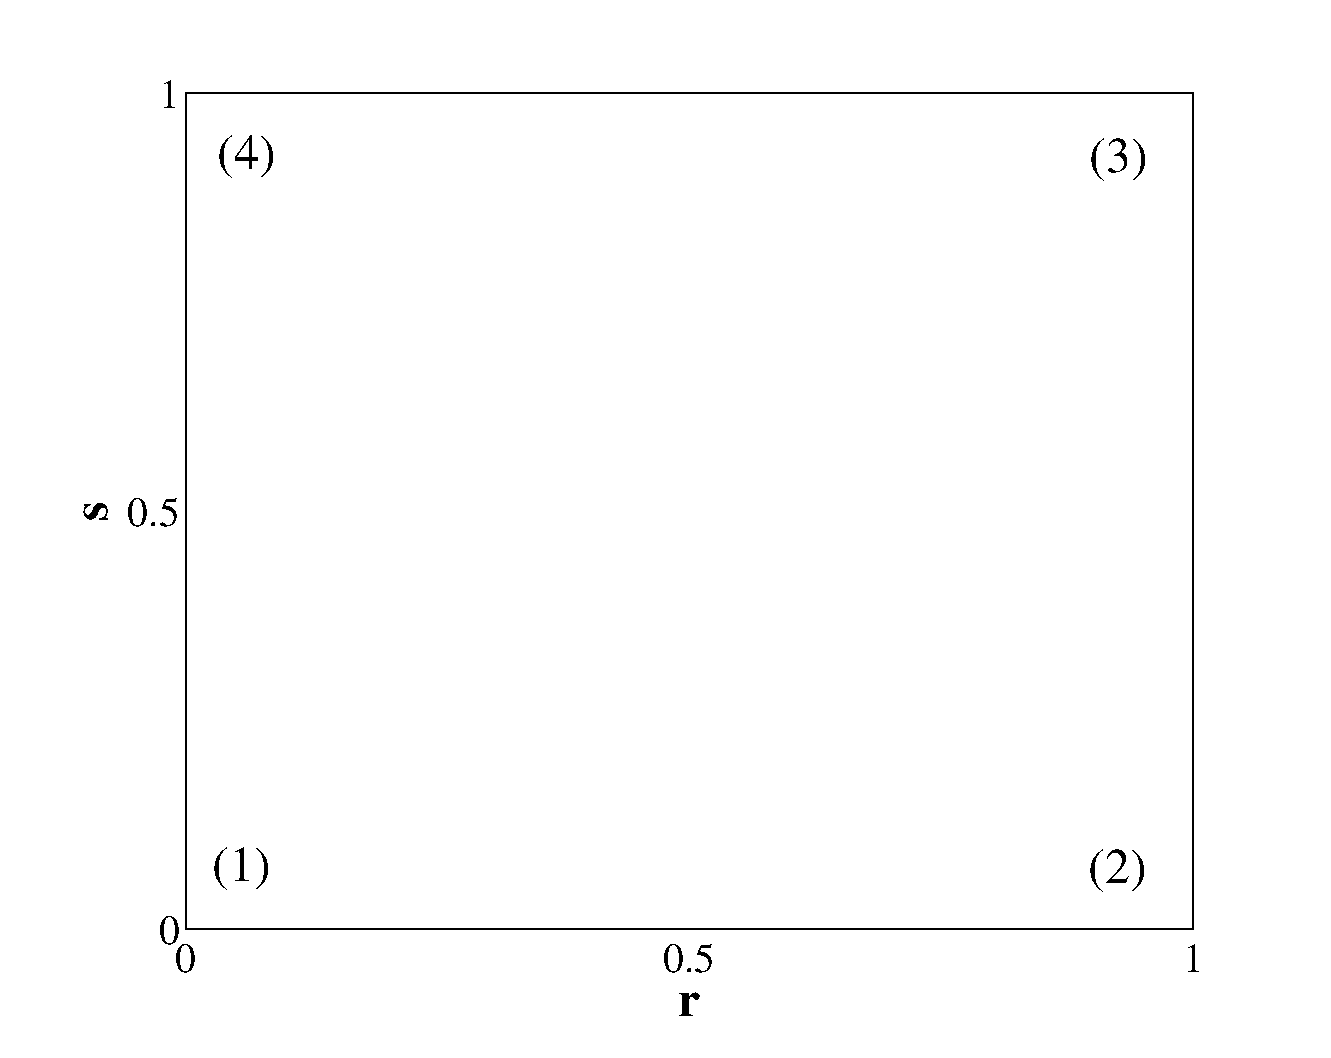
\includegraphics[width=\textwidth]{figures/sec_BF/unit_square_linear.eps}
		\caption{}
	\end{subfigure}
	\hfill
	\begin{subfigure}[b]{0.45\textwidth}
		\centering
		\label{subfig::unit_cube}
		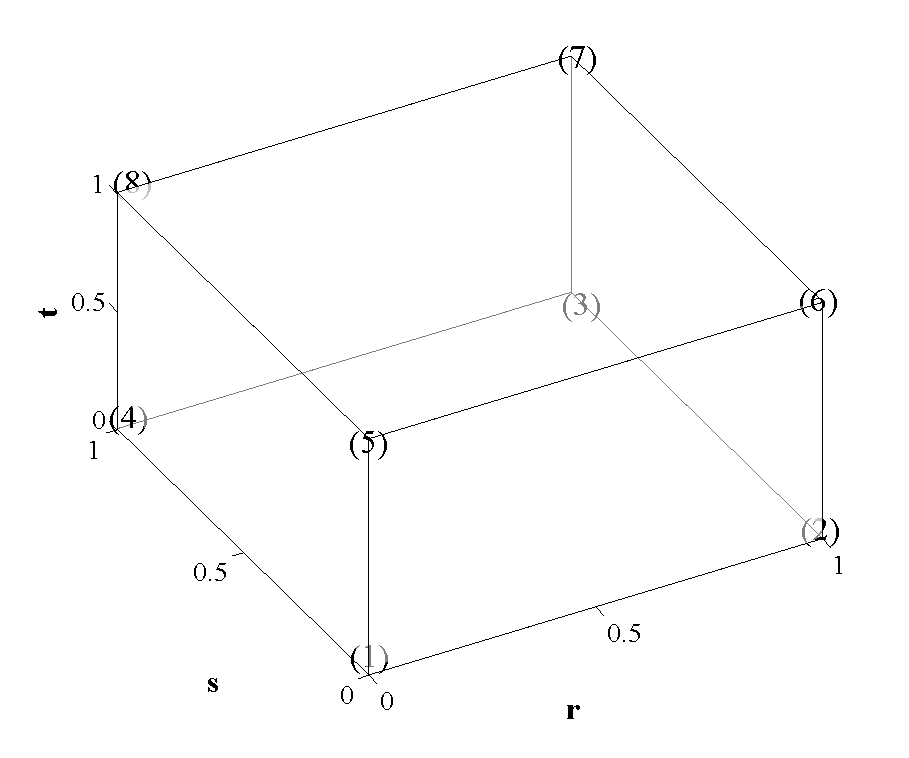
\includegraphics[width=\textwidth]{figures/sec_BF/unit_cube_linear.eps}
		\caption{}
	\end{subfigure}
\caption{Vertex structure for the (a) unit square and (b) unit cube.}
\label{fig::BF_3D_unit_tet_cube}
\end{figure}

\begin{equation}
\label{eq::3D_lin_basis_functions}
\begin{aligned}
	b_1(r,s) & = 1-r-s-t \\
	b_2(r,s) & = r \\
	b_3(r,s) & = s \\
	b_4(r,s) & = t
\end{aligned}
\end{equation}

\noindent and

\begin{equation}
\label{eq::TriL_basis_functions}
\begin{aligned}
	b_1(r,s,t) & = (1-r)(1-s)(1-t) \\
	b_2(r,s,t) & = r(1-s)(1-t) \\
	b_3(r,s,t) & = rs(1-t) \\
	b_4(r,s,t) & = (1-r)s(1-t) \\
	b_5(r,s,t) & = (1-r)(1-s)t \\
	b_6(r,s,t) & = r(1-s)t \\
	b_7(r,s,t) & = rst \\
	b_8(r,s,t) & = (1-r)st \\
\end{aligned}
\end{equation}

%%%%%%%%%%%%%%%%%%%%%%%%%%%%%%%%%%%%%%%%%%%%%%%%%%%
%%%   SubSection - PWL
\subsection{3D Piecewise Linear (PWL) Basis Functions}
\label{sec::BF_3D_PWL}

The 3D PWL basis functions share a similar form to the 2D PWL basis functions.

\begin{equation}
\label{eq::PWL_3D}
	b_j (x,y,z)  = t_j  (x,y,z) + \sum_{f=1}^{F_j} \beta_f^j  t_f (x,y,z) + \alpha_j^K t_c  (x,y,z)
\end{equation}

\noindent $t_j$ is the standard 3D linear function with unity at vertex $j$ that linearly decreases to zero to the cell center, the face center for each face that includes vertex $j$, and each vertex that shares an edge with vertex $j$. $t_c$ is the 3D cell ``tent" function which is unity at the cell center and linearly decreases to zero to each cell vertex and face center. $t_f$ is the face "tent" function which is unity at the face center and linearly decreases to zero at each vertex on that face and the cell center. $\beta_{f,j}$ is the weight parameter for face $f$ touching cell vertex $j$, and $F_j$ is the number of faces touching vertex $j$. Like the previous work defining the PWLD method \cite{bailey2008phd}, we also choose to assume the cell and face weighting parameters are

\begin{equation}
\alpha_{K,j} = \frac{1}{N_K} \qquad \text{and} \qquad \beta_{f,j} = \frac{1}{N_f},
\label{eq::PWL_weight_vals}
\end{equation}

\noindent respectively, where $N_K$ is the number of vertices in cell $K$ and $N_f$ is the number of vertices on face $f$, which leads to constant values of $\alpha$ and $\beta$ for each cell and face, respectively. This assumption of the cell weight function holds for both 2D and 3D.

%%%%%%%%%%%%%%%%%%%%%%%%%%%%%%%%%%%%%%%%%%%%%%%%%%%
%%%   Section - Results
\section{Numerical Results}
\label{sec::BF_Results}

Now that we have presented several linear polygonal finite element basis sets along with the methodology to convert them to quadratic serendipity-like basis, we present several numerical problems to demonstrate our methodology. First, we demonstrate that the presented basis sets preserve the thick diffusion limit in Section \ref{sec::BF_Results_TDL}. Next, we present some convergence properties of the basis sets using the method of manufactured solutions (MMS) in Section \ref{sec::BF_Results_MMS}. We then present a searchlight problem and observe how the basis sets react with adaptive mesh refinement (AMR) to mitigate numerical dispersion through a vacuum in Section \ref{sec::BF_Results_SL}.


%%%%%%%%%%%%%%%%%%%%%%%%%%%%%%%%%%%%%%%%%%%%%%%%%%%
%%%   SubSection - Thick Diffusive Limit
\subsection{Transport Solutions in the Thick Diffusive Limit}
\label{sec::BF_Results_TDL}

We present our first numerical example by demonstrating that the various polygonal finite element basis sets satisfy the thick diffusion limit. 


\begin{equation}
\label{eq::BF_Results_TDL_scaling}
\begin{aligned}
	\sigma_t &\rightarrow \frac{\sigma_t}{\epsilon} \\
	\sigma_a &\rightarrow \epsilon \sigma_t\\
	\frac{Q_0}{4 \pi} &\rightarrow \epsilon \frac{Q_0}{4 \pi}
\end{aligned}
\end{equation}

\begin{equation}
\label{eq::BF_Results_TDL_scaled_trans_eq}
\vec{\Omega} \cdot \vec{\nabla} \Psi + \frac{\sigma_t}{\epsilon} \Psi = \sigma_t \left( \frac{1}{\epsilon} - \epsilon   \right)  \frac{\Phi}{4 \pi} + \epsilon \frac{Q_0}{4 \pi}
\end{equation}

\begin{equation}
\label{eq::BF_Results_TDL_scaled_diff_eq}
\epsilon \vec{\nabla} \cdot \frac{1}{3 \sigma_t}  \vec{\nabla} \Phi + \epsilon \sigma_t \Phi =  \epsilon Q_0
\end{equation}

\begin{equation}
\label{eq::BF_Results_TDL_normalized_eqs}
\begin{aligned}
\vec{\Omega} \cdot \vec{\nabla} \Psi + \frac{1}{\epsilon} \Psi &=  \left( \frac{1}{\epsilon} - \epsilon   \right)  \frac{\Phi}{4 \pi} +  \frac{\epsilon}{4 \pi} \\
\frac{\epsilon}{3} {\nabla}^2 \Phi &+ \epsilon  \Phi =  \epsilon 
\end{aligned}
\end{equation}


%%%%%%%%%%%%%%%%%%%%%%%%%%%%%%%%%%%%%%%%%%%%%%%%%%%
%%%   SubSection - MMS
\subsection{Analytical Transport Solutions by the Method of Manufactured Solutions}
\label{sec::BF_Results_MMS}

The next numerical example we investigate involves the method of manufactured solutions (MMS). 

%%%%%%%%%%%%%%%%%%%%%%%%%%%%%%%%%%%%%%%%%%%%%%%%%%%
%%%   SubSection - Searchlight Problem
\subsection{Searchlight Problem}
\label{sec::BF_Results_SL}

The next example models a beam or searchlight. Similar problems were investigated in Dedner and Vollm{\"o}ller \cite{dedner2002adaptive} and Wang and Ragusa \cite{wang2011standard}. In this problem, an incident beam of neutrons is shined onto a small portion of a boundary, propagates through a vacuum, and then exits through a small portion of a different boundary. As the beam propagates through the vacuum, the spatial discretization causes radiation outflow through all downwind cell faces. This leads to numerical dispersion and will cause to beam to artificially broaden.

In this problem, we investigate an $\mathbb{R}^2$ domain of size $[0,1]^2$. The radiation enters the left boundary between $0.2 \leq y \leq 0.4$ with an un-normalized angular direction of $[1,0.4]$. For this chosen direction, the radiation beam would analytically leave the right boundary between $0.6 \leq y \leq 0.8$. This means that any radiation leaving the right boundary for all other $y$ values is due to the numerical dispersion of the beam.

We investigated this problem using several of the 2D polygonal basis functions as outlined in Section \ref{sec::BF_2D} as well as 

%%%%%%%%%%%%%%%%%%%%%%%%%%%%%%%%%%%%%%%%%%%%%%%%%%%
%%%   Section - Conclusions
\section{Conclusions}
\label{sec::BF_Conclusions}

In this chapter, we have presented 







